\section{Alignment with the ISO/IEC 27560 standard}
\label{sec:iso_27560}

ISO and IEC are an international standardisation body with technical committees established to specify requirements and guidelines for particular technical activities.
The ISO/IEC 27560 standard on `Privacy technologies -- Consent record information structure' \textit{``specifies an interoperable, open and extensible information structure for recording PII principals' consent to PII processing''}~\citep{isoiec_jtc_1sc_27_isoiec_2023}.
It outlines requirements and recommendations regarding the utilisation of consent receipts and consent records related to the processing of personally identifiable information (PII).
Its objectives include facilitating (i) a consent record for data controllers, (ii) the exchange of consent details among information systems, and (iii) the management of the consent life cycle.
Figure~\ref{fig:iso_27560} showcases the information elements of the consent record and receipt structure specified in the ISO/IEC 27560 standard, including examples of what information should be entered in each field.

\begin{figure}[ht]
    \centering
    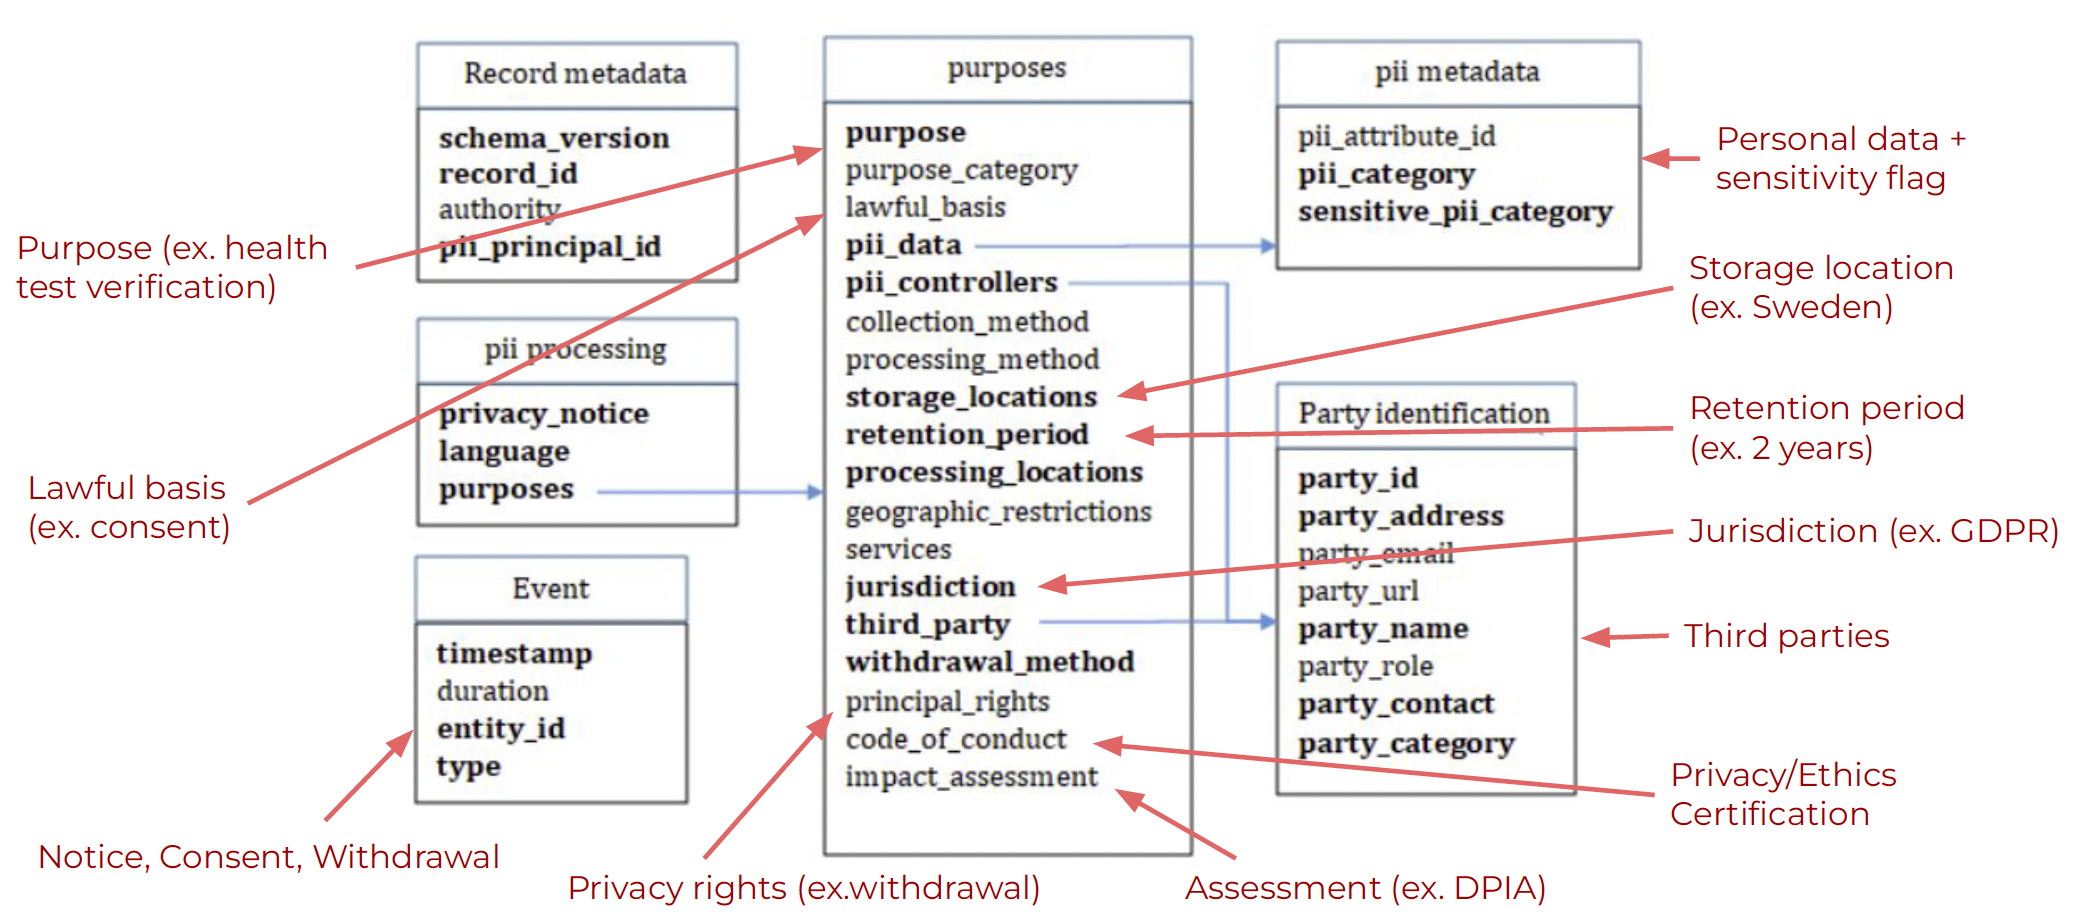
\includegraphics[width=1\linewidth]{figures//chapter-4/iso_27560.png}
    \caption{Elements of the ISO/IEC 27560 consent record and receipt structure~\citep{isoiec_jtc_1sc_27_isoiec_2023}.}
    \label{fig:iso_27560}
\end{figure}

Most of the fields illustrated in this Figure can be represented using the OAC-based data agreements proposed in Section~\ref{sec:oac}, as well as the existing ODRL and DPV specifications and the proposed work on PLASMA and the rights exercise extension described in Section~\ref{sec:plasma} and~\ref{sec:rights_exercising}.
The `record metadata' elements \textbf{record\_id}, \textbf{pii\_principal\_id}, and \textbf{authority} can be instantiated using the \texttt{odrl:uid}, the \texttt{dpv:hasDataSubject}, and the \texttt{dpv:hasAuthority} properties, and the `pii processing' terms \textbf{privacy\_notice}, and \textbf{language} with PLASMA's notice terms and \texttt{odrl:language} left operand.
Furthermore, the `Event' terms can be modelled using PLASMA and DPV's concepts to model notices, consent statuses, and logs of processing activities, and records of right exercise activities with the work proposed in Section~\ref{sec:rights_exercising}.
The `Party identification' elements can be modelled using the \texttt{oac:Entity} placeholder that should be set on agreement policies for assigners and assignees, as well as for constraints on which recipients can get access to the data, which can then be specifically defined with DPV's legal entity concepts as well as PLASMA entity terms to specify specific decentralised/Solid-related roles.
Contact-related information can also be modelled with DPV's \texttt{hasName}, \texttt{hasContact} and \texttt{hasAddress} properties.
Moreover, most `purposes' terms can already be modelled with existing and proposed work, such as the proposed OAC terms to restrict purposes, legal bases, data types, processing operations, including collection, or services, as well as existing ODRL temporal and spatial constraints, and DPV's concepts related rights, jurisdictions or impact assessments.
Additionally, DPV, and in particular its personal data extension, can be used to specify the categories of personal or sensitive personal data being used and specified in the standard as `pii metadata'.

As such, it is possible to check that the existing and proposed work is aligned with the ISO/IEC 27560 standard for consent records and hence can be used to fulfil almost all of the recommended elements.
Future work can be focused on providing machine-readable codes of conduct, and more comprehensive event specifications, e.g., data holders' permission terms proposed in the DGA.